\documentclass[aspectratio=169,12pt]{beamer}
\usetheme{Madrid}
\usecolortheme{dolphin}
\usefonttheme{professionalfonts}
\setbeamertemplate{navigation symbols}{}
\setbeamertemplate{footline}{}

\usepackage[T1]{fontenc}
\usepackage[utf8]{inputenc}
\usepackage{graphicx}
\usepackage{amsmath,amssymb}
\usepackage{hyperref}
\usepackage{siunitx}
\usepackage{physics}
\usepackage{braket}

\title{Module A5: Circuits et portes logiques}
\author{JAMOTTE Maxime, SCHOONEN Cédric}
\institute{Digital Learning Hub}
\date{}

\begin{document}

\begin{frame}
  \titlepage
\end{frame}

% \begin{frame}{Table des matières}
%   \tableofcontents
% \end{frame}

% \section{}

\begin{frame}{Objectifs}
  \begin{itemize}
  \item Circuits logiques classiques\\~\\
  \item Circuits quantiques (+ B2)\\~\\
  \item Circuit pour construire un état quantique depuis $\ket{00...0}$\\~\\
  \item Modèle de calcul: circuit -> exécution sur QPU -> résultats de mesures
  \end{itemize}
\end{frame}

\begin{frame}{Circuits de portes logiques classiques}
  \begin{itemize}[<+->]
    \setlength{\itemsep}{0.55em}
    \item Bits classiques: 0 ou 1; les portes transforment ces bits.
    \item Exemples clés : NOT, AND, OR, XOR, NAND (porte universelle).
    \item On enchaîne ces portes pour construire des circuits logiques.
  \end{itemize}
  \vfill
  \only<2->{%
    \centering
    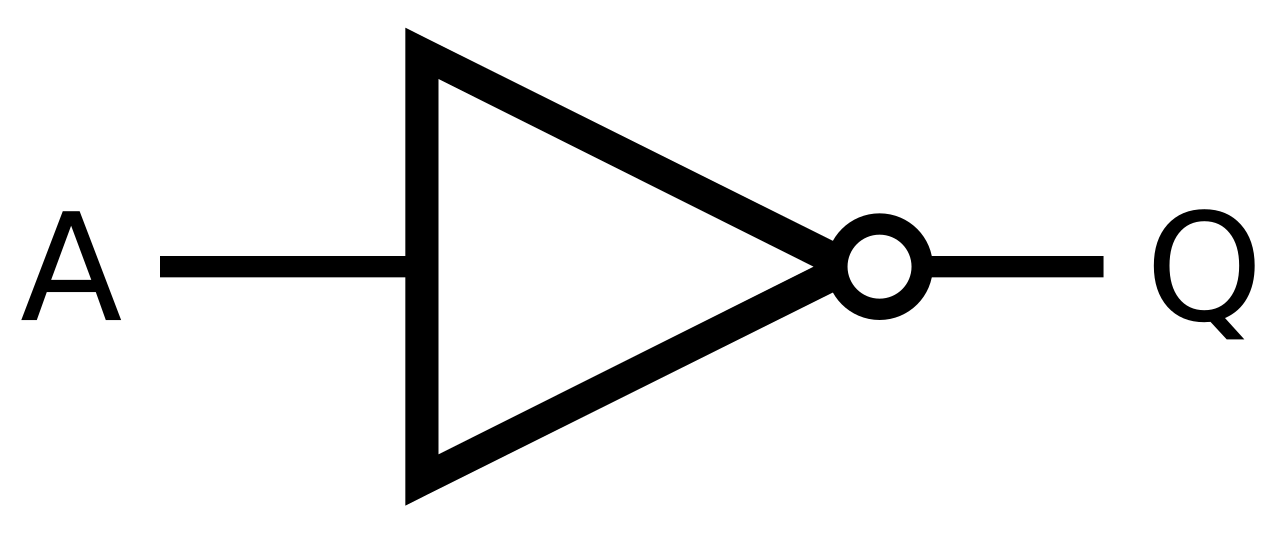
\includegraphics[height=1.1cm]{figures/NOT.png}\hspace{0.3cm}
    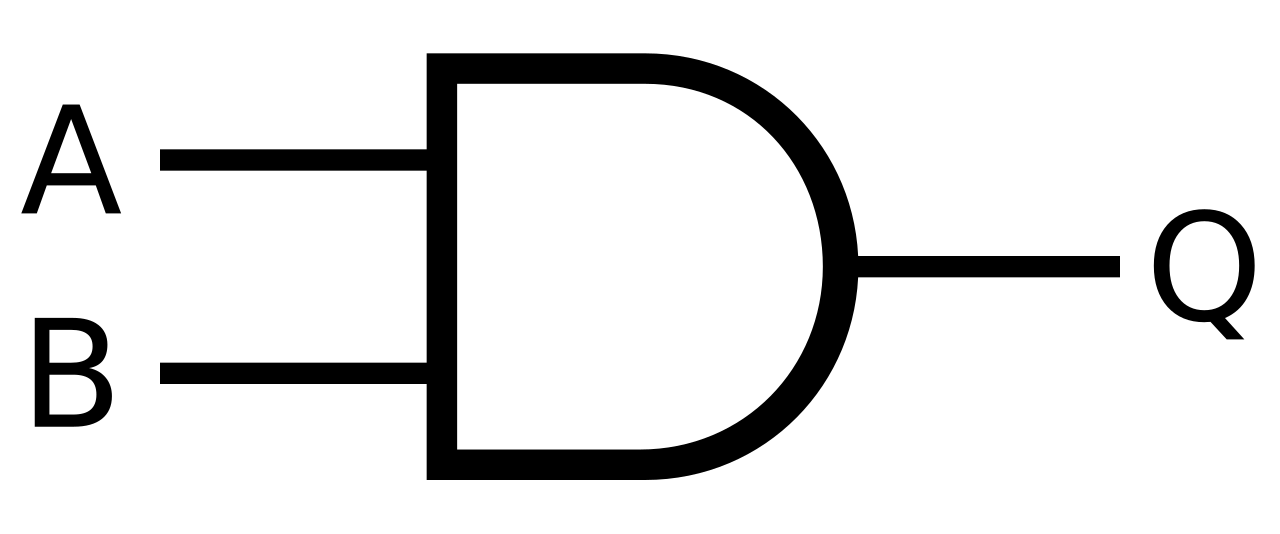
\includegraphics[height=1.1cm]{figures/AND.png}\hspace{0.3cm}
    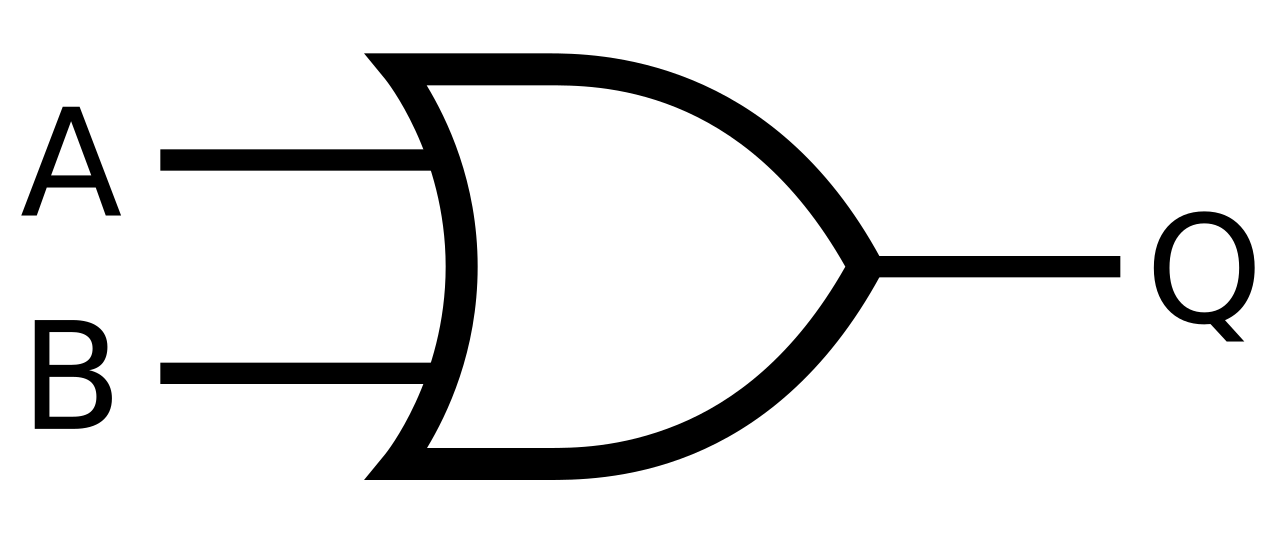
\includegraphics[height=1.1cm]{figures/OR.png}\hspace{0.3cm}
    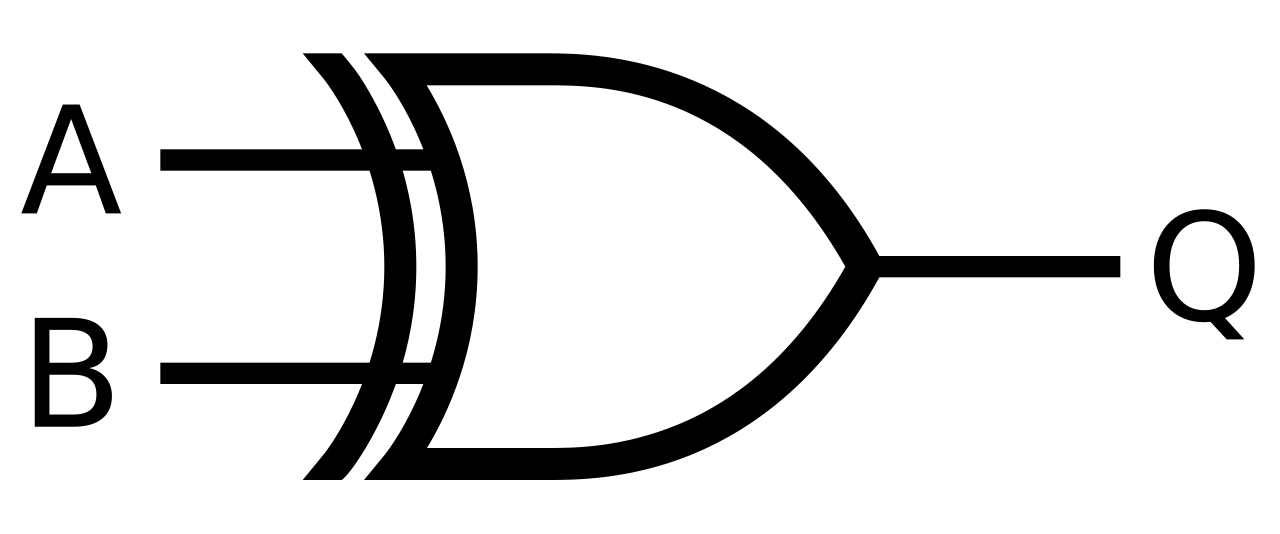
\includegraphics[height=1.1cm]{figures/XOR.png}\hspace{0.3cm}
    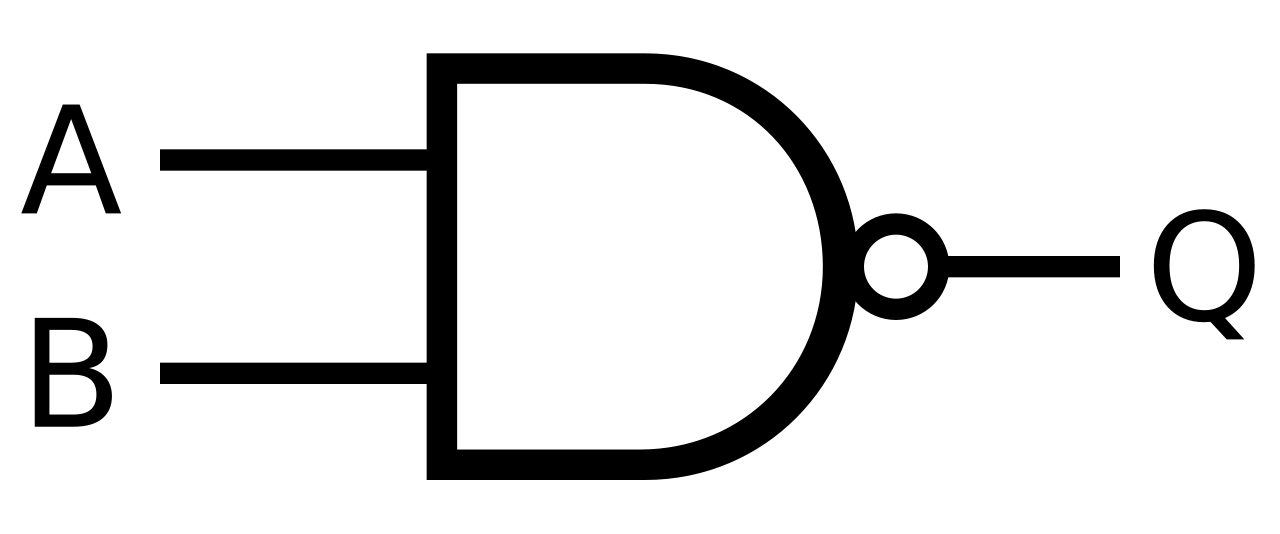
\includegraphics[height=1.1cm]{figures/NAND.png}
  }
\end{frame}

\begin{frame}{Table de vérité (rappel)}
  \centering
  \renewcommand{\arraystretch}{1.4}
  \begin{tabular}{l c c c}
    \textbf{Porte} & \textbf{Symbole} & \textbf{Expression} & \textbf{Description} \\\hline
    NOT   & $\lnot A$ & inverse & $1\leftrightarrow 0$ \\
    AND   & $A\cdot B$ & $1$ si $A=1$ et $B=1$ & porte "multiplication" \\
    OR    & $A + B$ & $1$ si $A=1$ ou $B=1$ & porte "addition" \\
    XOR   & $A \oplus B$ & $1$ si $A\neq B$ & "ou exclusif" \\
    NAND  & $\lnot(A\cdot B)$ & inverse de AND & base universelle \\
  \end{tabular}
\end{frame}



\begin{frame}{Table de vérité XOR / AND}
  \centering
  \renewcommand{\arraystretch}{1.4}
  \begin{tabular}{c c | c | c}
    $A$ & $B$ & $A\ \mathbf{XOR}\ B$ & $A\ \mathbf{AND}\ B$ \\\hline
    0 & 0 & 0 & 0 \\
    0 & 1 & 1 & 0 \\
    1 & 0 & 1 & 0 \\
    1 & 1 & 0 & 1 \\
  \end{tabular}
\end{frame}

\begin{frame}{Exemple de circuit classique}
  \begin{itemize}[<+->]
    \item Enchaînement de portes pour additionner deux bits (avec report).
    \item Chaque fil transporte un bit, chaque symbole applique une porte.
  \end{itemize}
  \vfill
  \centering
  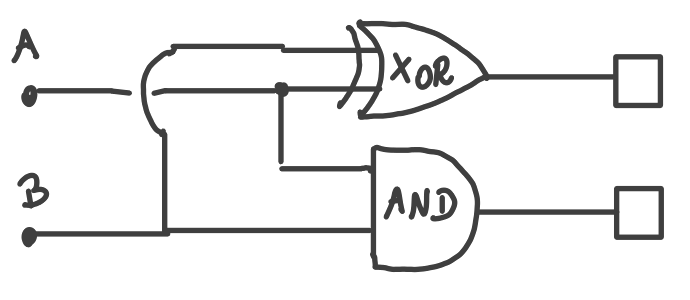
\includegraphics[width=0.65\textwidth]{figures/addition_circuit2.png}
\end{frame}

\begin{frame}{Circuits quantiques, mesures et simulations (module B2)}
  \begin{itemize}
    \item Construire un circuit quantique avec des portes à 1 et 2 qubits\\~\\
    \item Simuler un circuit et interpréter les résultats de mesure\\~\\
  \end{itemize}
\end{frame}

\begin{frame}{Exécuter un circuit sur un QPU}
  \begin{itemize}
    \item Création d'un circuit\\~\\
    \item Choix de la platfomre d'exécution (cloud ou local)
    \begin{enumerate}
      \vspace{0.5em}
    \item `QPU` : exécute le circuit sur un processeur quantique IBM réel via Qiskit Runtime, avec bruit matériel;
    \item `FakeQPU` : imite un QPU IBM à partir d'un snapshot (topologie, portes natives, propriétés des qubits) pour tester la transpilation et une simulation bruitée;
    \item `Aer` : simule le circuit en local avec `AerSimulator`, rapidement et avec plusieurs méthodes de simulation, avec ou sans modèle de bruit
    \end{enumerate}~\\
    \item Transpilation du circuit pour l'adapter au QPU\\~\\
    ~\\~\\~\\
  \end{itemize}
\end{frame}

\begin{frame}{Transpilation}
  \begin{columns}[T]
    \begin{column}{0.55\textwidth}
      \vspace{1cm}
      \centering
      
\includegraphics[width=\textwidth]{figures/grover.png}
    \end{column}
    \begin{column}{0.4\textwidth}
      \centering
      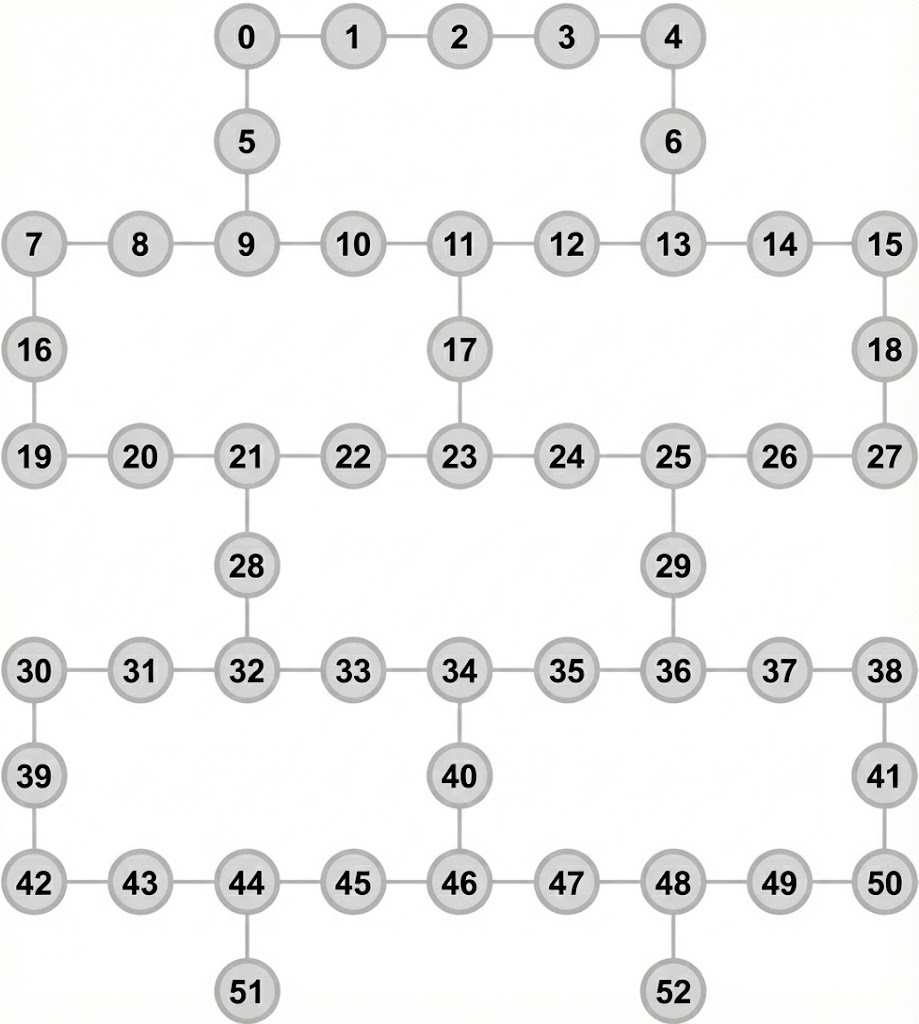
\includegraphics[width=\textwidth]{figures/qubits_layout.jpg}
    \end{column}
  \end{columns}
\end{frame}

\begin{frame}{Transpilation : Six Étapes}
  \begin{columns}[T]
    \begin{column}{0.58\textwidth}
      \small
      \vspace{-0.7em}
      \begin{enumerate}
        \setlength{\itemsep}{0.3em}
        \item \textbf{Init}: Réduction des opérations multi-qubits en portes à 1 et 2 qubits (Optionnel)
        \item \textbf{Layout}: Assignation des qubits physiques
        \item \textbf{Routing}: Insertion de portes SWAP pour déplacer les états quantiques entre qubit (NP-difficile, algorithme aléatoire)
        \item \textbf{Translation}: Conversion de toutes les portes vers le jeu d'instructions natif (ISA)
        \item \textbf{Optimization}: Remplacement ou élimination de portes logiques où c'est possible
        \item \textbf{Scheduling}: Insertion de délais (Optionnel)
      \end{enumerate}
    \end{column}
    \begin{column}{0.4\textwidth}
      \centering
      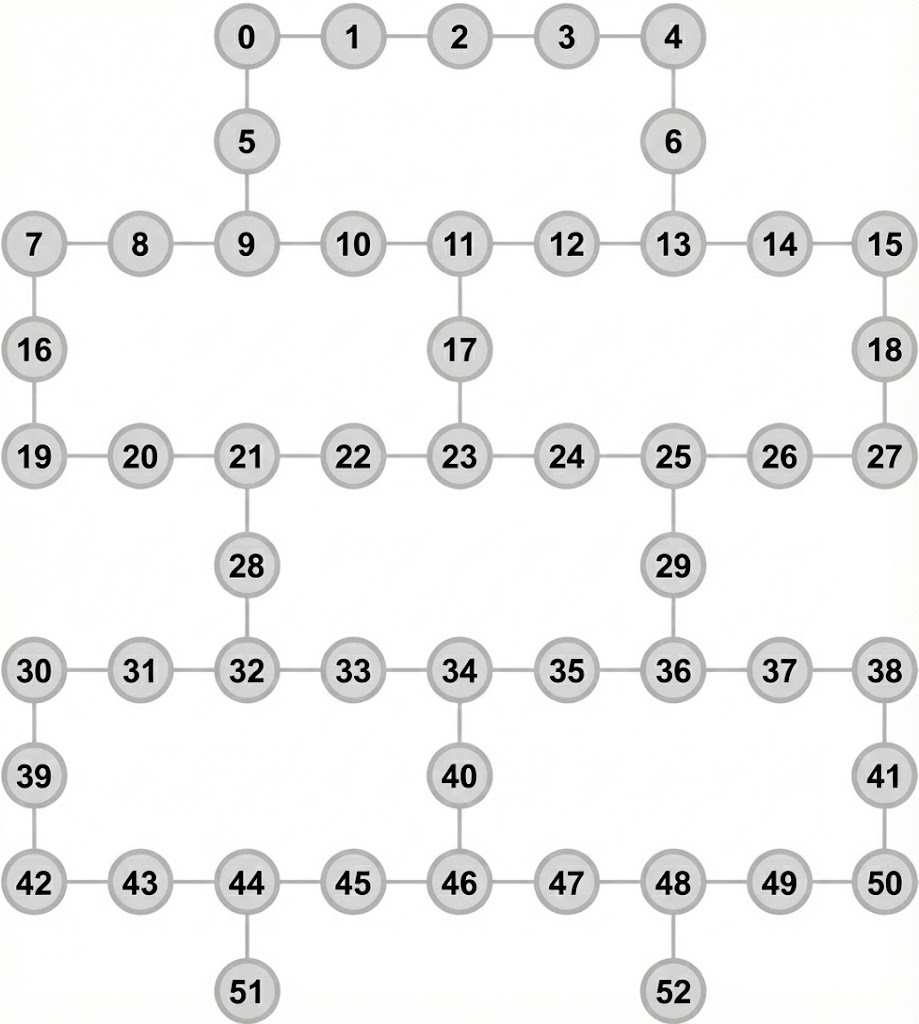
\includegraphics[width=\textwidth]{figures/qubits_layout.jpg}
    \end{column}
  \end{columns}
\end{frame}

\begin{frame}{Transpilation: Niveaux d'Optimisation}
  \small
  \begin{description}
    \setlength{\itemsep}{1.5em}
    \item[\textbf{Niveau 1}:] Combination matricielle des portes à un qubit,\\ élimination des portes CNOT redondantes
    
    \item[\textbf{Niveau 2}:] Analyse de commutation pour éliminer davantage de redondances
    
    \item[\textbf{Niveau 3}:] Optimisation des sous-blocs à deux qubits identifiés dans le circuit\\ (reconstruit une matrice unitaire équivalente)
  \end{description}
\end{frame}

\begin{frame}{Exécuter un circuit sur un QPU (module B3)}
  \begin{itemize}
    \item Création d'un circuit\\~\\
    \item Choix de la platfomre d'exécution (Fake ou QPU)\\~\\
    \item Transpilation du circuit pour l'adapter à la topologie du QPU\\~\\
    \item Exécution du circuit \\~\\
    \item Récupération et analyse des résultats de mesure
  \end{itemize}
\end{frame}



% \begin{frame}{États et opérateurs à 1 qubit (voir JN)}
%   \begin{itemize}
%     \item Circuits quantiques créés avec \texttt{QuantumCircuit} puis convertis en \texttt{Statevector.from\_circuit}.\\~\\
%     \item Visualisation rapide des circuits avec \texttt{qc.draw('mpl')}.
%   \end{itemize}
% \end{frame}

% \begin{frame}{Circuits quantiques à 1 qubit (voir JN)}
%   \begin{itemize}
%     \item Porte de Hadamard ($H$)
%     \\~\\
%     \item Porte NOT ($X$)
%   \end{itemize}
%   \vfill
%   \begin{columns}[T,onlytextwidth]
%     \column{0.48\textwidth}
%     \centering
%     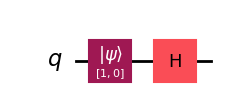
\includegraphics[width=0.8\linewidth]{figures/gate_hadamard.png}
%     \\[-0.3em]\footnotesize Circuit \texttt{Qiskit} pour $H$
%     \column{0.48\textwidth}
%     \centering
%     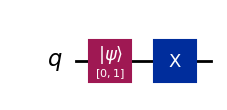
\includegraphics[width=0.8\linewidth]{figures/gate_x.png}
%     \\[-0.3em]\footnotesize Circuit \texttt{Qiskit} pour $X$
%   \end{columns}
% \end{frame}

% \begin{frame}{Porte Hadamard: circuit et action (voir JN)}
%   \begin{columns}[T,onlytextwidth]
%     \column{0.5\textwidth}
%     \centering
%     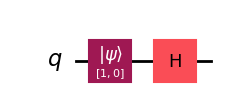
\includegraphics[width=0.75\linewidth]{figures/gate_hadamard.png}
%     \\[-0.3em]\footnotesize Circuit \texttt{Qiskit} pour $H$
%     \column{0.5\textwidth}
%     \small
%     \[
%       H = \frac{1}{\sqrt{2}}
%       \begin{pmatrix}
%         1 & 1 \\
%         1 & -1
%       \end{pmatrix},
%       \qquad
%       H\ket{0} = \tfrac{1}{\sqrt{2}}(\ket{0} + \ket{1})
%     \]
%     Superposition égale des deux états de base.
%   \end{columns}
% \end{frame}

% \begin{frame}{Porte $X$ : circuit et action (voir JN)}
%   \begin{columns}[T,onlytextwidth]
%     \column{0.5\textwidth}
%     \centering
%     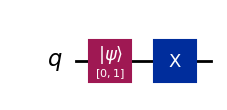
\includegraphics[width=0.75\linewidth]{figures/gate_x.png}
%     \\[-0.3em]\footnotesize Circuit \texttt{Qiskit} pour $X$
%     \column{0.5\textwidth}
%     \small
%     \[
%       X =
%       \begin{pmatrix}
%         0 & 1 \\
%         1 & 0
%       \end{pmatrix},
%       \qquad
%       X\ket{0} = \ket{1}
%     \]
%     Permutation des amplitudes: $|0\rangle \leftrightarrow |1\rangle$.
%   \end{columns}
% \end{frame}

% \begin{frame}{Exercice 4.1 : $H$ sur \(\ket{1}\) (voir JN)}
%   \begin{columns}[T,onlytextwidth]
%     \column{0.55\textwidth}
%     \begin{itemize}[<+->]
%       \item Point de départ : \(\ket{1} = \begin{pmatrix}0\\ 1\end{pmatrix}\).\\~\\
%       \item Appliquer la porte de Hadamard : \(H\ket{1} = \tfrac{1}{\sqrt{2}}(\ket{0} - \ket{1})\).\\~\\
%       \item Modifier l'état initial dans le code (remplacer \(\ket{0}\) par \(\ket{1}\)) et observer la nouvelle superposition.
%     \end{itemize}
%     \column{0.45\textwidth}
%     \centering
%     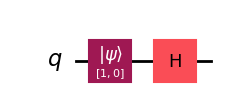
\includegraphics[width=0.8\linewidth]{figures/gate_hadamard.png}
%   \end{columns}
% \end{frame}

% \begin{frame}{Exercice 4.1 : $X$ puis $H$ sur \(\ket{0}\) (voir JN)}
%   \begin{columns}[T,onlytextwidth]
%     \column{0.55\textwidth}
%     \begin{itemize}[<+->]
%       \item Point de départ : \(\ket{0}\).\\~\\
%       \item Chaîne d'opérations : \(H X \ket{0} = H\ket{1} = \tfrac{1}{\sqrt{2}}(\ket{0} - \ket{1})\).\\~\\
%     \end{itemize}
%     \column{0.45\textwidth}
%     \centering
%     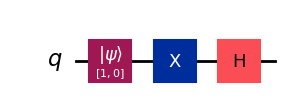
\includegraphics[width=0.8\linewidth]{figures/gate_x_then_h.png}
%   \end{columns}
% \end{frame}

% \begin{frame}{Exercice 4.2 : $H$ puis $X$ sur \(\ket{0}\) (voir JN)}
%   \begin{columns}[T,onlytextwidth]
%     \column{0.55\textwidth}
%     \begin{itemize}[<+->]
%       \item Point de départ : \(\ket{0} = \begin{pmatrix}1\\ 0\end{pmatrix}\).\\~\\
%       \item Chaîne d'opérations : \(X H \ket{0} = X \big(\tfrac{1}{\sqrt{2}}(\ket{0} + \ket{1})\big) = \tfrac{1}{\sqrt{2}}(\ket{0} + \ket{1})\).\\~\\
%       \item Construire le circuit (H suivi de X), visualiser et vérifier l'état final dans le notebook.
%       \item Comparer avec l'exercice 4.1 pour voir que l'ordre des portes change le résultat (non-commutativité).
%     \end{itemize}
%     \column{0.45\textwidth}
%     \centering
%     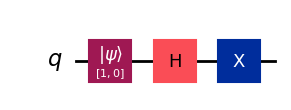
\includegraphics[width=0.8\linewidth]{figures/gate_h_then_x.png}
%   \end{columns}
% \end{frame}



\begin{frame}{Fin du module}
\end{frame}

\end{document}
